% Foliensatz: "AFu-Kurs nach DJ4UF" von DK0TU, Amateurfunkgruppe der TU Berlin
% Lizenz: CC BY-NC-SA 3.0 de (http://creativecommons.org/licenses/by-nc-sa/3.0/de/)
% Autoren: Sebastian Lange <dl7bst@dk0tu.de>

\documentclass[aspectratio=169]{beamer}

\usepackage[ngerman]{babel} % deutsche Worttrennung etc.
\usepackage[utf8]{inputenc} % UTF8 Text

\usepackage[super, comma, numbers, square, sort]{natbib}

\usepackage{hyperref}       % Hyperref Package für bessere Referenzen (todo)
\hypersetup{
	colorlinks=false,       %   false: boxed links; true: colored links
    %linkcolor=white,       %   color of internal links (change box color with linkbordercolor)
    citecolor=red,          %   color of links to bibliography
    filecolor=white,        %   color of file links
    urlcolor=blue           %   color of external links
}

\usepackage{multirow}
\usepackage{wasysym}  % Math Symbols like \permil
%\usepackage{colortbl}
%\usepackage{subscript}
%\usepackage{caption}
%\usepackage{setspace}
%\usepackage{xcolor}        % benutze CodeListe

% Footnote
%\usepackage{hanging}
%
%\setbeamertemplate{footnote}{%
%  \hangpara{2em}{1}%
%  \makebox[2em][l]{\insertfootnotemark}\footnotesize\insertfootnotetext\par%
%}


%\usepackage{pgf}
%\usepackage{tikz}
%\usetikzlibrary{arrows,automata}
%\usetikzlibrary{positioning}
%
%\tikzset{
%    state/.style={
%           rectangle,
%           rounded corners,
%           draw=black, very thick,
%           minimum height=2em,
%           minimum width=2pt,
%           inner sep=2pt,
%           text centered,
%           },
%}

%\usepackage{listings}
%\lstset{basicstyle=\small, numberstyle=\tiny, extendedchars=true, numbers=left, numbersep=5pt}
%\lstset{showtabs=false, showspaces=false, showstringspaces=false}
%%\lstset{backgroundcolor=\color{white!75!lightgray}, , frame=single}
%%\lstset{backgroundcolor=\color{white}}
%%\lstset{backgroundcolor=none}
%\lstset{keywordstyle=\color{blue!50!gray},  identifierstyle=\color{black}}
%\lstset{commentstyle=\color{green!50!gray}, stringstyle=\color{red!50!gray}}
%\lstset{language=C, fontadjust=true, tabsize=2, breaklines=true}
%\lstset{backgroundcolor=\color{white!75!lightgray}, caption=\lstname, frame=single}
%\lstset{emphstyle=\color{black}\fbox}
%
%% Keine "Listing:"-Caption
%\captionsetup{labelformat=empty,labelsep=none}
%
%% für mathematische Umgebungen
%\usepackage{amsmath,amsfonts,amssymb}
%
%\lstdefinestyle{Bash}{
%language=Bash,
%frame=single,
%rulecolor=\color{black},
%backgroundcolor=\color{gray!50},
%keywordstyle=\color{black},
%identifierstyle=,
%commentstyle=\color{black},
%stringstyle=\color{magenta!65!white},
%showstringspaces=false,
%basicstyle=\footnotesize\ttfamily\color{black},
%numbers=none,
%breaklines=true,
%captionpos=b
%}

%\usepackage{listings}
%
%\lstdefinestyle{basic}{
%    captionpos=t,%
%    basicstyle=\footnotesize\ttfamily,%
%    numberstyle=\tiny,%
%    numbers=left,%
%    stepnumber=1,%
%    frame=single,%
%    showspaces=false,%
%    showstringspaces=false,%
%    showtabs=false,%
%    %
%    keywordstyle=\color{blue},%
%    identifierstyle=,%
%    commentstyle=\color{gray},%
%    stringstyle=\color{magenta}%
%}



% fließende Boxen haben keinen Abstand
%\fboxsep0mm

% inkludiere Creative Commons Helper
%%%%%%%%%%%%%%%%%%%%%%%%%%%%%%%%%%%%%%%%%%%%%%%%%%%%%%%%%%%%%%%%
%% ccBeamer 0.1, 2007-07-02                                   %%
%% Written by Sebastian Pipping <webmaster@hartwork.org>      %%
%% ---------------------------------------------------------- %%
%% Licensed under Creative Commons Attribution-ShareAlike 3.0 %%
%% http://creativecommons.org/licenses/by-sa/3.0/             %%
%%%%%%%%%%%%%%%%%%%%%%%%%%%%%%%%%%%%%%%%%%%%%%%%%%%%%%%%%%%%%%%%


%% Images
\newcommand{\CcImageBy}[1]{%
	
\includegraphics[scale=#1]{texdata/creative_commons/cc_by_30.pdf}%
}
\newcommand{\CcImageCc}[1]{%
	
\includegraphics[scale=#1]{texdata/creative_commons/cc_cc_30.pdf}%
}
\newcommand{\CcImageDevNations}[1]{%
	
\includegraphics[scale=#1]{texdata/creative_commons/cc_dev_nations_30.pdf}%
}
\newcommand{\CcImageNc}[1]{%
	
\includegraphics[scale=#1]{texdata/creative_commons/cc_nc_30.pdf}%
}
\newcommand{\CcImageNd}[1]{%
	
\includegraphics[scale=#1]{texdata/creative_commons/cc_nd_30.pdf}%
}
\newcommand{\CcImagePd}[1]{%
	
\includegraphics[scale=#1]{texdata/creative_commons/cc_pd_30.pdf}%
}
\newcommand{\CcImageSa}[1]{%
	
\includegraphics[scale=#1]{texdata/creative_commons/cc_sa_30.pdf}%
}
\newcommand{\CcImageSampling}[1]{%
	
\includegraphics[scale=#1]{texdata/creative_commons/cc_sampling_30.pdf}%
}
\newcommand{\CcImageSamplingPlus}[1]{%
	
\includegraphics[scale=#1]{texdata/creative_commons/cc_sampling_plus_30.pdf}%
}


%% Groups
\newcommand{\CcGroupBy}[2]{% zoom, gap
	\CcImageCc{#1}\hspace*{#2}\CcImageBy{#1}%
}
\newcommand{\CcGroupByNc}[2]{% zoom, gap
	\CcImageCc{#1}\hspace*{#2}\CcImageBy{#1}\hspace*{#2}\CcImageNc{#1}%
}
\newcommand{\CcGroupByNcNd}[2]{% zoom, gap
	\CcImageCc{#1}\hspace*{#2}\CcImageBy{#1}\hspace*{#2}\CcImageNc{#1}\hspace*{#2}\CcImageNd{#1}%
}
\newcommand{\CcGroupByNcSa}[2]{% zoom, gap
	\CcImageCc{#1}\hspace*{#2}\CcImageBy{#1}\hspace*{#2}\CcImageNc{#1}\hspace*{#2}\CcImageSa{#1}%
}
\newcommand{\CcGroupByNd}[2]{% zoom, gap
	\CcImageCc{#1}\hspace*{#2}\CcImageBy{#1}\hspace*{#2}\CcImageNd{#1}%
}
\newcommand{\CcGroupBySa}[2]{% zoom, gap
	\CcImageCc{#1}\hspace*{#2}\CcImageBy{#1}\hspace*{#2}\CcImageSa{#1}%
}
\newcommand{\CcGroupDevNations}[2]{% zoom, gap
	\CcImageCc{#1}\hspace*{#2}\CcImageDevNations{#1}%
}
\newcommand{\CcGroupNcSampling}[2]{% zoom, gap
	\CcImageCc{#1}\hspace*{#2}\CcImageNc{#1}\hspace*{#2}\CcImageSampling{#1}%
}
\newcommand{\CcGroupPd}[1]{% zoom
	\CcImagePd{#1}%
}
\newcommand{\CcGroupSampling}[1]{% zoom
	\CcImageSampling{#1}%
}
\newcommand{\CcGroupSamplingPlus}[1]{% zoom
	\CcImageSamplingPlus{#1}%
}


%% Text
\newcommand{\CcLongnameBy}{Attribution}
\newcommand{\CcLongnameByNc}{Attribution-NonCommercial}
\newcommand{\CcLongnameByNcNd}{Attribution-NoDerivs}
\newcommand{\CcLongnameByNcSa}{Attribution-NonCommercial-ShareAlike}
\newcommand{\CcLongnameByNd}{Attribution-NoDerivs}
\newcommand{\CcLongnameBySa}{Attribution-ShareAlike}

\newcommand{\CcNote}[1]{% longname
	This work is licensed under the \textit{Creative Commons #1 3.0 License}.%
}


% generelles Thema auswählen
\usetheme{Goettingen} %Berlin spart ohne Sidebar allerdings angenehm Platz
% AnnArbor | Antibes | Bergen | Berkeley | Berlin | Boadilla | boxes | CambridgeUS | Copenhagen | Darmstadt | default | Dresden | Frankfurt | Goettingen | Hannover | Ilmenau | JuanLesPins | Luebeck | Madrid | Malmoe | Marburg | Montpellier | PaloAlto | Pittsburgh | Rochester | Singapore | Szeged | Warsaw

% Farben wählen
\usecolortheme{beetle}
% beaver | beetle | crane | default | dolphin | dove | fly | lily | orchid | rose | seagull | seahorse | sidebartab | structure | whale | wolverine

% Setze alle Farben auf Grau und Weiß
%\definecolor{craneorange}{RGB}{64,64,64}
%\definecolor{craneblue}{RGB}{255,255,255}

% Schriftart wählen
\usefonttheme{default}
% default | professionalfonts | serif | structurebold | structureitalicserif | structuresmallcapsserif

% Innere Themen(Kopf-, Fuß-, Sidebar usw)
%\useinnertheme{default}
\useinnertheme{circles}
% default | inmargin | rectangles | rounded | circles

% Äußere Themen (Anordnung der inneren, grenzen der Folien etc.)
\useoutertheme{infolines}
% default | infolines | miniframes | shadow | sidebar | smoothbars | smoothtree | split | tree

% Deaktiviere Navigations-Symbole ({} -> leer)
\setbeamertemplate{navigation symbols}{}
%\setbeamertemplate{navigation symbols}{\large \ifnum \insertframenumber <10 0\fi\insertframenumber/\inserttotalframenumber\vspace*{0.2ex}}

% Zeige ein Hintergrundbild
\setbeamertemplate{background canvas}{
        \hspace*{-2.0cm}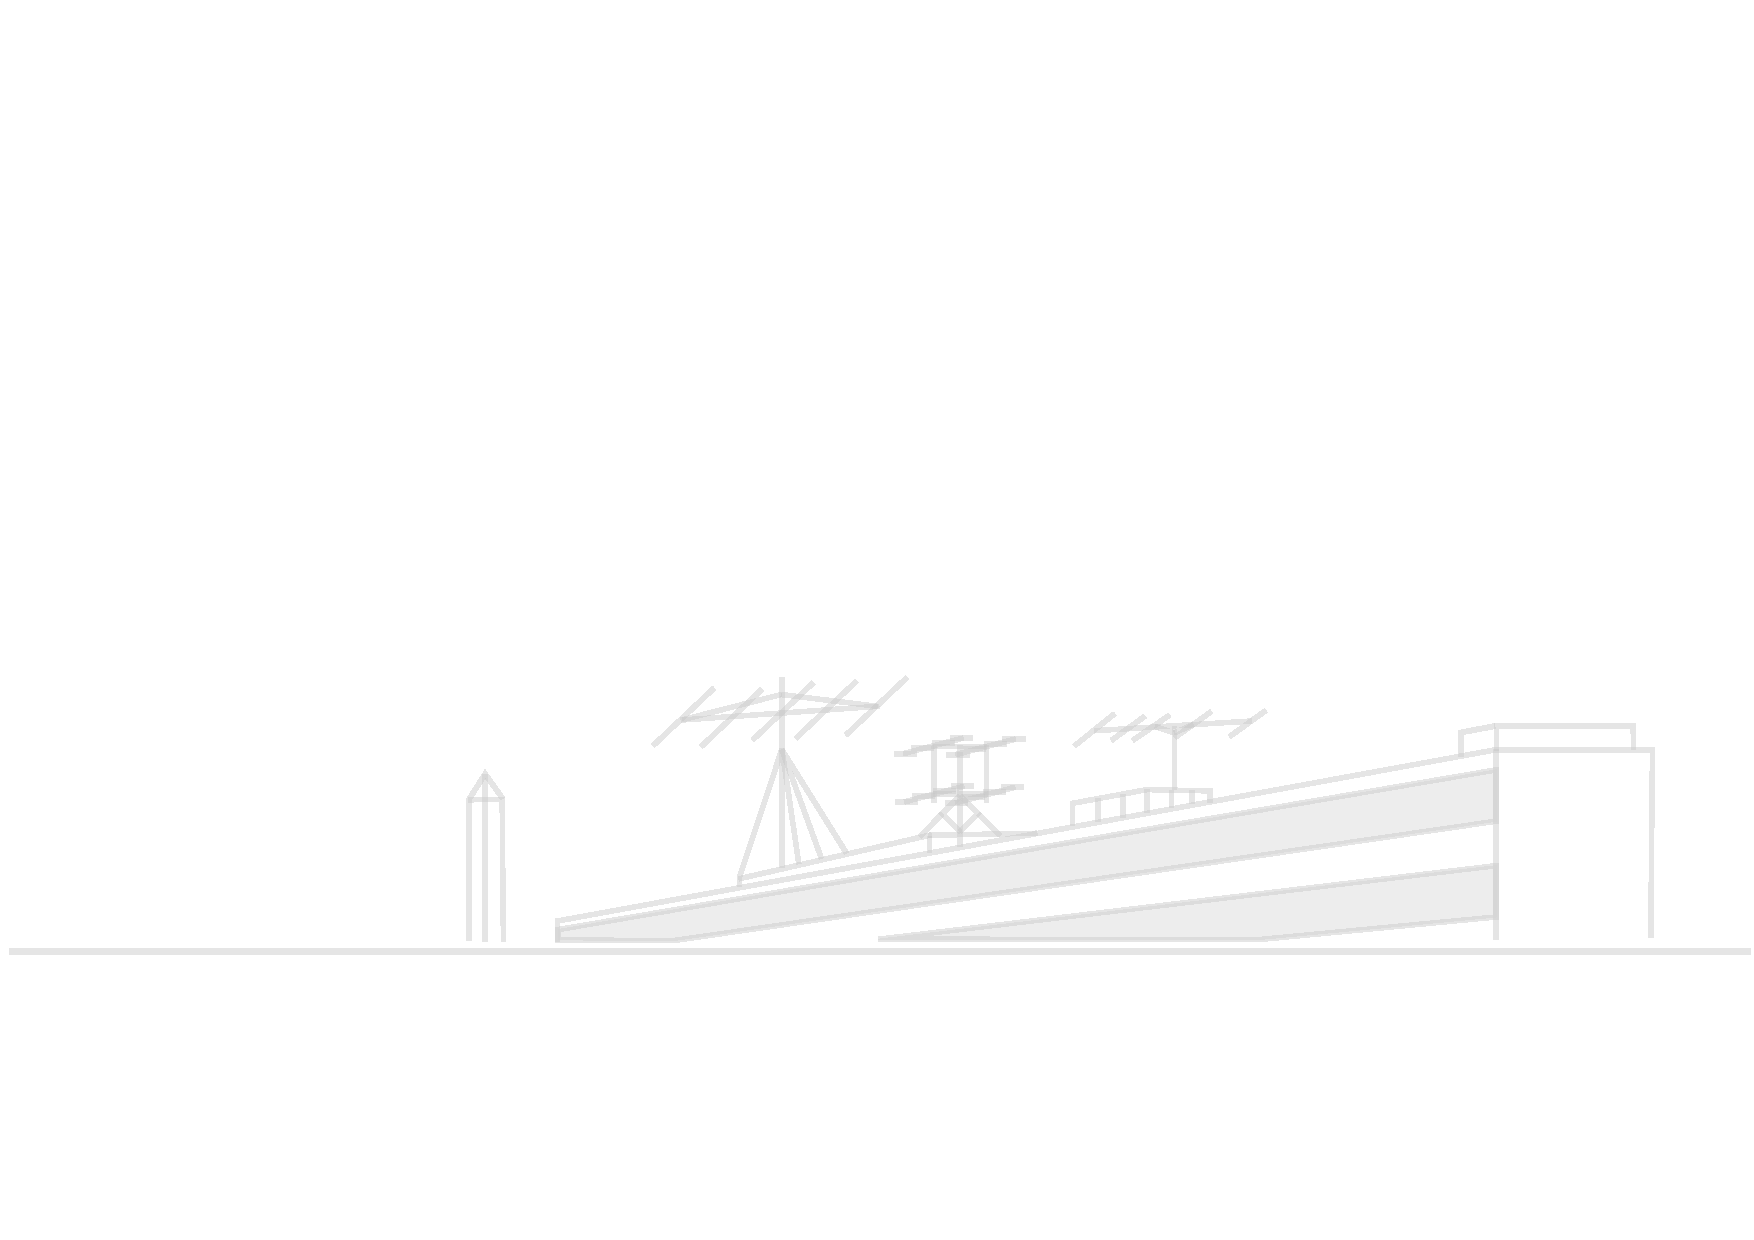
\includegraphics[width=17.8cm]{texdata/dk0tu_rooftop_background.pdf}
}

% Foliennummer einfügen
\setbeamertemplate{footline}[frame number]
%\setbeamertemplate{footline}{}

% Ändere das Zeichen vor jedem item
%\setbeamertemplate{itemize item}{\color{craneorange}$\blacktriangleright$}
%\setbeamertemplate{itemize subitem}{\color{craneorange}$\triangleright$}
%\setbeamertemplate{itemize subsubitem}{\color{craneorange}$\blacktriangleright$}

% Ändert die Blöcke 
\setbeamertemplate{blocks}[rounded][shadow=true]
% default | rounded [shadow=true|false]

%
% Eigene Kommandos
%

% Hack to get natbib and beamer working together. "The beamer user guide suggests
% that only the manual bibliography entry approach is supported"
% on some system it works out of the box, sometimes you need the hack :-(
% so check it --dl7bst
\ifdefined\newblock
    \relax
\else
    \newcommand{\newblock}{}
\fi

% \includedia command to generate png out of a dia file
% NEEDS installed dia and pdflatex option --shell-escape
\newcommand{\includedia}[1]{
    \immediate\write18{/usr/bin/dia #1.dia -e #1_diatmp.png -t png}
}

% RICHIG GROSSER FONT!
\newfont{\bigfont}{cmr10 at 144pt}
\newfont{\smallfont}{cmr10 at 8pt}

% Römische Ziffern
\makeatletter
\newcommand{\rmnum}[1]{\romannumeral #1}
\newcommand{\Rmnum}[1]{\expandafter\@slowromancap\romannumeral #1@}
\makeatother

% Schwarze Überschrift
%\setbeamercolor{frametitle}{fg=black}
%\setbeamercolor{title}{fg=black}

% Item- und Box-Farben
\definecolor{deepBlue}{HTML}{000066}
\setbeamercolor{itemize item}{fg=deepBlue}
\setbeamercolor{itemize subitem}{fg=deepBlue}
\setbeamercolor{description item}{fg=deepBlue}
\setbeamercolor{block title}{fg=deepBlue!100, bg=blue!15}
\setbeamercolor{block body}{fg=black, bg=blue!5}
\setbeamercolor{block title alerted}{fg=deepBlue, bg=red!75}
\setbeamercolor{block body alerted}{fg=black, bg=red!15}
\setbeamercolor*{block title example}{fg=blue!50, bg=blue!10}
\setbeamercolor*{block body example}{fg= blue, bg=blue!5}

%\setbeamercolor{section in head/foot}{parent=palette primary}
%\setbeamercolor{subsection in head/foot}{parent=palette secondary}
%\setbeamercolor{sidebar}{fg=darkblue,bg=yellow!90!orange}
%\setbeamercolor{title in sidebar}{fg=darkblue}
%\setbeamercolor{author in sidebar}{fg=darkblue}
%\setbeamercolor{section in sidebar}{fg=darkblue!10!black}
%\setbeamercolor{subsection in sidebar}{fg=darkblue!50!black}

% Titlepage Infos
\title{AFu-Kurs nach DJ4UF}
\author[DKØTU]{DKØTU\\ \footnotesize{Amateurfunkgruppe der TU Berlin}}
\institute[DKØTU]{\url{http://www.dk0tu.de} }

% PDF-Eigenschaften
\subject{DK0TU-Amateurfunkkurs nach DJ4UF}
\keywords{Amateurfunk Kurs HAM Radio Course CC-BY-NC-SA OpenSource TU Berlin DK0TU}

\subtitle{Technik Klasse E 00: \\
          Curriculum \& Organisatorisches \\[2em]}
\date{Stand 11.09.2017}
 \begin{document}

\begin{frame}
    \titlepage
    \vfill
    \begin{center}
        \ccbyncsaeu\\
        {\tiny This work is licensed under the \em{Creative Commons Attribution-NonCommercial-ShareAlike 3.0 License}.}\\[0.5ex]
         \tiny Amateurfunkgruppe der Technische Universität Berlin (AfuTUB), DKØTU
         %\includegraphics[scale=0.5]{img/DK0TU_Logo.pdf}
    \end{center}
\end{frame}


% TODO weitere Infos ergänzen? Was ist Afu (CQ-Talk) in die Präsi mit einflechten?

\section{Vorweg}

\begin{frame}

    \begin{columns}[c]
        \column[c]{3.5cm}
        \begin{center}
            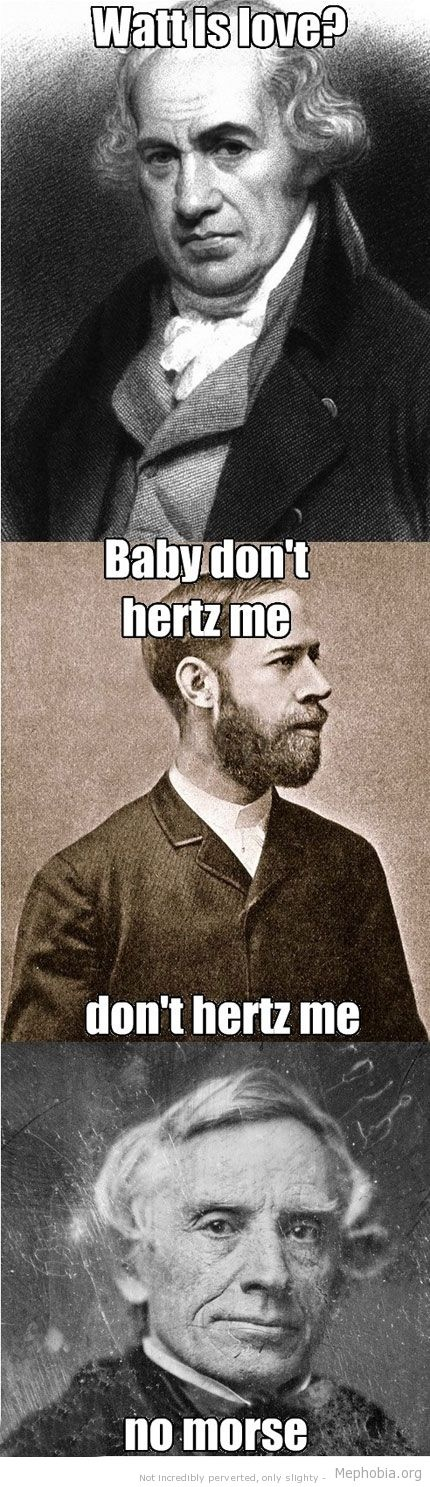
\includegraphics[height=1\textheight]{e00/watthertzmorse.jpg}
            \tiny \hyperlink{refs}{\cite{meph}}
        \end{center}
        \column{6.5cm}
            \only<1>{Vorweg: Kennt ihr die drei?}
            \only<2-4>{
                \begin{itemize}
                    \item James Watt (1736-1819), \\ schottischer Erfinder
                    \item Heinrich Hertz (1857-1894), \\ deutscher Physiker
                    \item Samuel F. B. Morse (1791-1872), \\ US-amerikanischer Erfinder
                \end{itemize}
            }
            \only<3-4>{\bigskip Telegrafie vor der Frequenz? \\[1em]}
            \only<4>{$\rightarrow$ klar, Telegrafie lange Zeit leitungsgebunden.}
    \end{columns}

\end{frame}

\subsection{Amateurfunk}

\begin{frame}
  \frametitle{Amateurfunk}

  \begin{itemize}
    \item ca. 65.000 Funkamateure in Deutschland
    \item davon ca. 35.000 im Deutschen Amateur-Radio-Club e.V. (DARC)
    \item weltweit ca. 3 Mio Funkamateure (genaue Zahl unklar)
  \end{itemize}

  \begin{exampleblock}{Wichtiger Unterschied zum Walkie-Talkie}
    Nicht das Gerät, sondern die Person wird geprüft!
  \end{exampleblock}

  \begin{itemize}
    \item Erlaubnis zum Selbstbau
    \item bestimmte Frequenzen sind ausschließlich für den Amateurfunk
  \end{itemize}
\end{frame}

\begin{frame}
  \frametitle{Vielfalt}

  \begin{exampleblock}{}
    Amateurfunk ist nicht ein Hobby, sondern viele
  \end{exampleblock}

  Basteln, Gespräche, Technik, DXpeditionen, Berge, Inseln, Schlösser, Naturschutzgebiete, Sport, Campen, Flohmarkt, Vorträge, Jugendarbeit, \ldots alles dabei!
\end{frame}

\subsection{D23}

\begin{frame}
  \frametitle{Was ist der D23?}

  Offizieller Titel: "`Delta 23 Freunde des CCC"'

  \begin{itemize}
    \item Ein "`Ortsverband"' im DARC
    \item Eigentlich an einen Ort gebunden, aber wir sind Hacker
    \item Eingetragen als Interessensgemeinschaft
    \item Wir treffen uns beim CCC oder auf seinen Veranstaltungen
    \item Zufälligerweise im "`Distrikt Delta"', also Berlin, des DARC angesiedelt
  \end{itemize}

  Die Chaoswelle sind die Amateurfunkfreunde des CCC auch ohne Mitgliedschaft im D23\footnote{Jetzt ist alles klar, oder?}.
\end{frame}

\subsection{CCCB}

\begin{frame}
  \frametitle{Der CCCB}

  \begin{itemize}
    \item Lokaler Erfa-Kreis des Chaos Computer Clubs
    \item Ihr seid in den Clubräumen
    \item Am Montagabend gibt es seit zwei Jahren Amateurfunk
    \item Vor vielen Jahren gab es schon mal Amateurfunktreffen im CCCB
  \end{itemize}
\end{frame}

\begin{frame}
  \frametitle{Clubraum}

  \begin{itemize}
    \item ca. 200qm zentral gelegen seit 1997
    \item Wohnzimmer/Vortragsraum
      \begin{itemize}
        \item Beleuchtung und Beschallung
        \item Matemat
        \item Barbereich
      \end{itemize}
    \item Küche
    \item Sanitäre Anlagen
    \item Keller
      \begin{itemize}
        \item Mitgliedsbereich
        \item Werkstatt und Labor
        \item Chillout Lounge mit Konsolenstrang
      \end{itemize}
  \end{itemize}
\end{frame}

\subsection{Vergangenheit}
\begin{frame}
  \frametitle{Bisherige Kurse}

  \begin{itemize}
    \item Vorläufer 2013 und 2014 in der AfRA mit 4 bis 10 Teilnehmenden
    \item 2015 mit 30 Teilnehmenden zu Beginn im CCCB mit dem Foliensatz von DK\O TU
    \item nach dem Kurs wöchentliche Amateurfunktreffen
    \item 2016 wieder im CCCB mit 35 Teilnehmenden
  \end{itemize}
\end{frame}


\section{Der Kurs}
\subsection{Überblick}

\begin{frame}
    \frametitle{Überblick}

    Dieser \textbf{Grundlagenkurs (Klasse E)} geht vom Abiturwissen
    \emph{Sekundarstufe II} aus (vgl. Curriculum \hyperlink{refs}{\cite{curr}}).

    \vspace{2em}

    %\includedia{e00/Zeitstrahl D23 2017}
    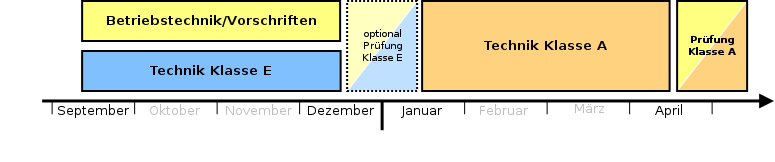
\includegraphics[width=1\textwidth]{o00/Zeitstrahl_D23_2017.png}\footnote{Für
    Hochschulen empfohlener Zeitplan \tiny (mit rein zufälliger Farbwahl \emph{HI})}

\end{frame}

\subsection{E vs. A}

\begin{frame}
    \frametitle{Klasse E vs. A}

    \textbf{Betriebstechnik und Vorschriften} sind äquivalent -- Klasse A geht
    viel tiefer in die Technik. \\[2em]

    Dafür "`winken"' als Zielprämie:

    \begin{itemize}
        \item mehr benutzbare TX-Frequenzen (alle AFu-Bänder)
        \item weitaus höhere Sendeleistungen bis zu $750W$
    \end{itemize}

\end{frame}

\subsection{Material}

\subsubsection[DARC-Lehrgang]{DARC Online-Lehrgang}

\begin{frame}
    \frametitle{DARC Online-Lehrgang}

    Wesentliche Materialgrundlage ist der deutschsprachige
    \emph{Amateurfunklehrgang \hyperlink{refs}{\cite{darc}} des
    DARC\footnote{Deutscher Amateur-Radio-Club}}.

    \begin{columns}[c]
        \column[c]{5cm}
        \begin{center}
            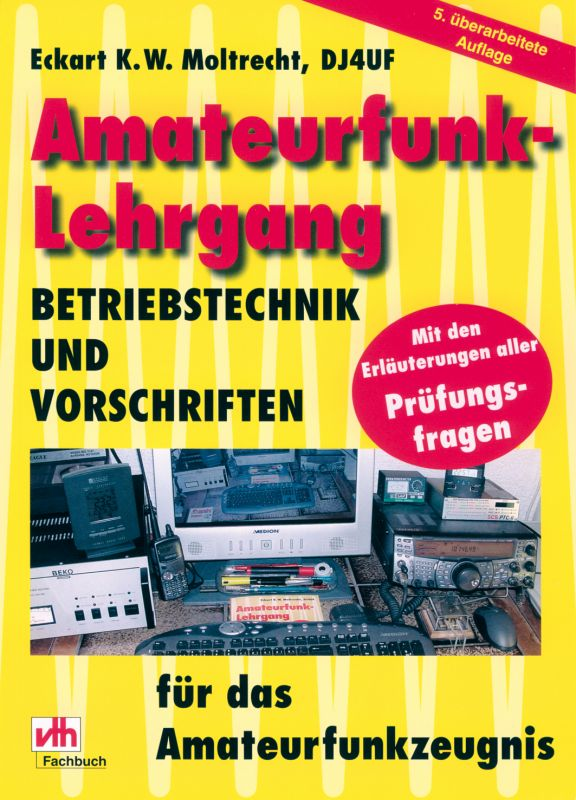
\includegraphics[width=0.7\textwidth]{e00/Amateurfunklehrgang-Betriebstechnik-und-Vorschriften.jpg}
            \tiny \hyperlink{refs}{\cite{darcv}}
        \end{center}
        \column{5cm}
            Inhaltlich entspricht dieser den von DJ4UF geschrieben Büchern - im
            Amaterfunk bekannt als "`Der Moltrecht"' \hyperlink{refs}{\cite{dj4uf}}
    \end{columns}

\end{frame}


\begin{frame}
    \frametitle{DARC Online-Lehrgang}

    Wesentliche Materialgrundlage ist der deutschsprachige
    \emph{Amateurfunklehrgang \hyperlink{refs}{\cite{darc}} des
    DARC\footnote{Deutscher Amateur-Radio-Club}}.

    \begin{columns}[c]
        \column[c]{5cm}
        \begin{center}
            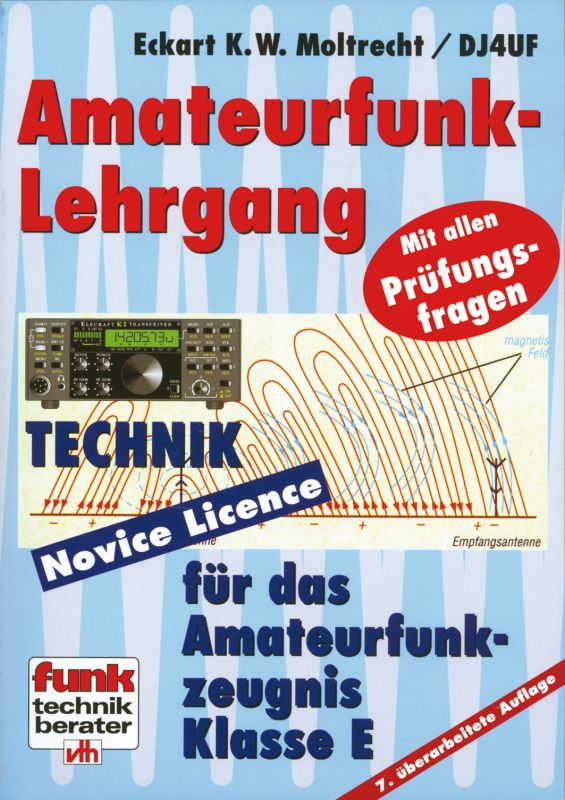
\includegraphics[width=0.7\textwidth]{e00/Amateurfunklehrgang-Technik-fuer-das-Amateurfunkzeugnis-Klasse-E.jpg}
            \tiny \hyperlink{refs}{\cite{darcv}}
        \end{center}
        \column{5cm}
        Mit Prüfungsziel \emph{Klasse A} kann \emph{nicht} auf das
        Klasse-E-Buch verzichtet werden, da oft auf das Klasse-E-Buch
        referenziert wird.
    \end{columns}

\end{frame}

\subsubsection{Fragenkataloge}

\begin{frame}
    \frametitle{Fragenkataloge}

    Dreh- und Angelpunkt aller Kurse: Der offizielle Fragenkatalog der
    Bundesnetzagentur\footnote{als Print z.B. direkt von der BNetzA oder als PDF im WWW}.

    \begin{columns}[c]
        \column[c]{3cm}
        \begin{center}
            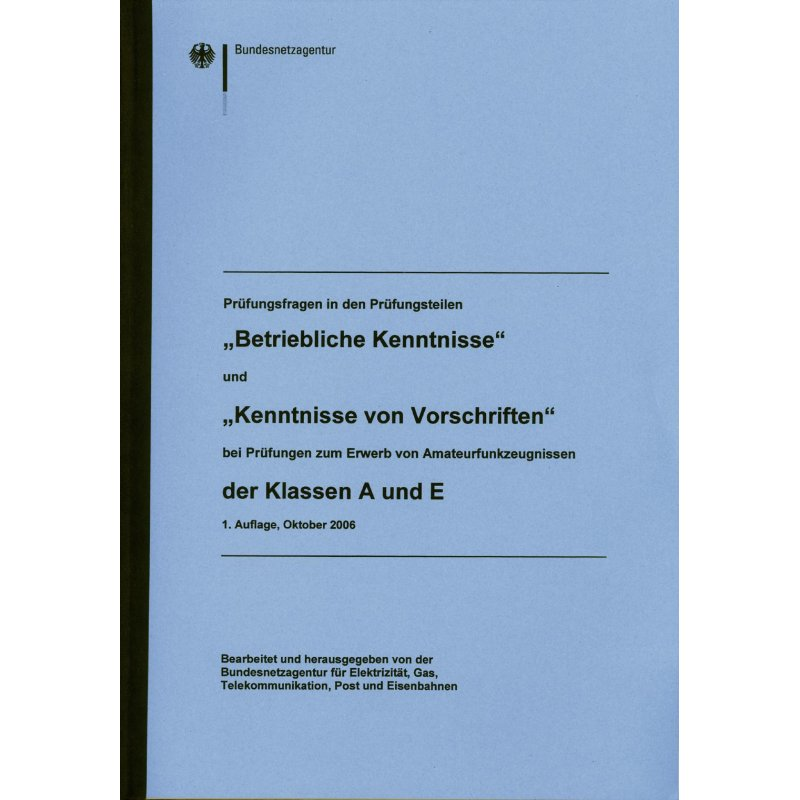
\includegraphics[height=0.6\textheight]{e00/Fragenkatalog-Klasse-A-und-E-Betriebliche-Kenntnisse-und-Kenntnisse-von-Vorschriften.jpg}
            \tiny \hyperlink{refs}{\cite{darcv}}
        \end{center}
        \column{7cm}
        \begin{itemize}
            \item digital verfügbar in verschiedenen Übungsprogrammen und
            Prüfungssimulatoren
            \item Empfehlung Offline-Tool: \emph{AFUTrainer} \hyperlink{refs}{\cite{afut}}
            \item Beste Empfehlung Browser-Tool: \emph{afutest} \hyperlink{refs}{\cite{afutest}} (von DD6EE, einem Kursteilnehmer 2016)
            \item Empfehlung Browser-Tool: \emph{AfuP} \hyperlink{refs}{\cite{afup}}
            \item auch kostenpflichtige Apps verfügbar
        \end{itemize}
    \end{columns}

\end{frame}

\begin{frame}
    \frametitle{Fragenkataloge}

    \begin{center}
        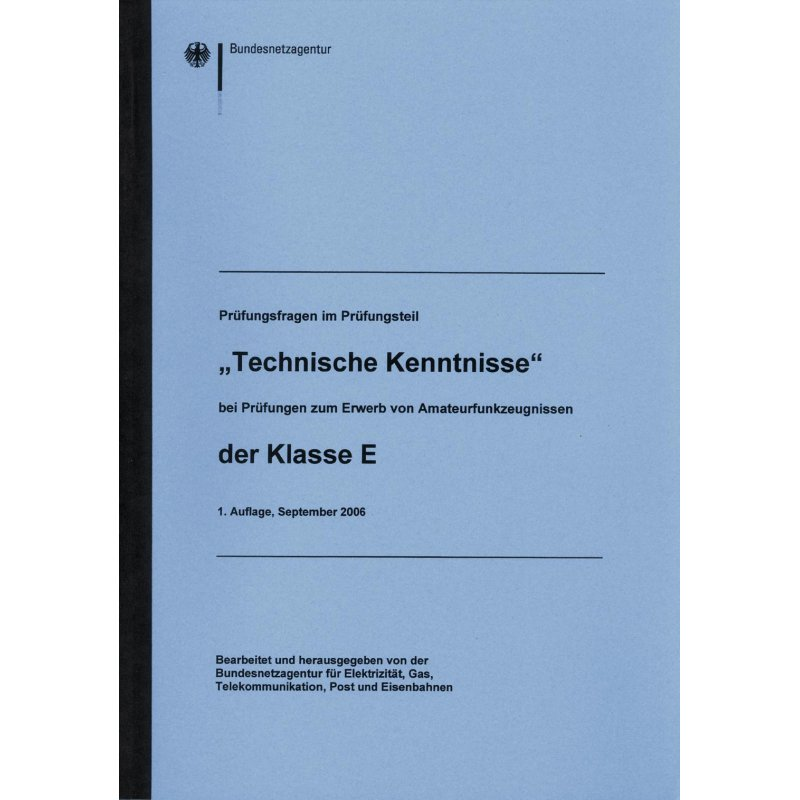
\includegraphics[height=0.7\textheight]{e00/Fragenkatalog-Klasse-E-Technische-Kenntnisse.jpg}
        \tiny \hyperlink{refs}{\cite{darcv}}
    \end{center}

    Auch dieser braucht für das Ziel \emph{Klasse A} nicht beachtet zu werden.

\end{frame}

\begin{frame}
    \frametitle{Formelsammlung}

    Wichtigster Auszug aus dem offiziellen Fragenkatalog der \emph{BNetzA} ist
    die Formelsammlung im Anhang. \\[3em]

    Auch wenn man sonst papierlos unterwegs ist:
    \textbf{Ausdrucken}\footnote{S.131-138 (PDF-Seiten 133-140)} lohnt sich!

\end{frame}

\subsection{Curriculum}

\subsubsection{Aufbau}

\begin{frame}
    \frametitle{Curriculum / Abhängigkeitsgraph}

    %\includedia{e00/Abhaengigkeitsgraph}
    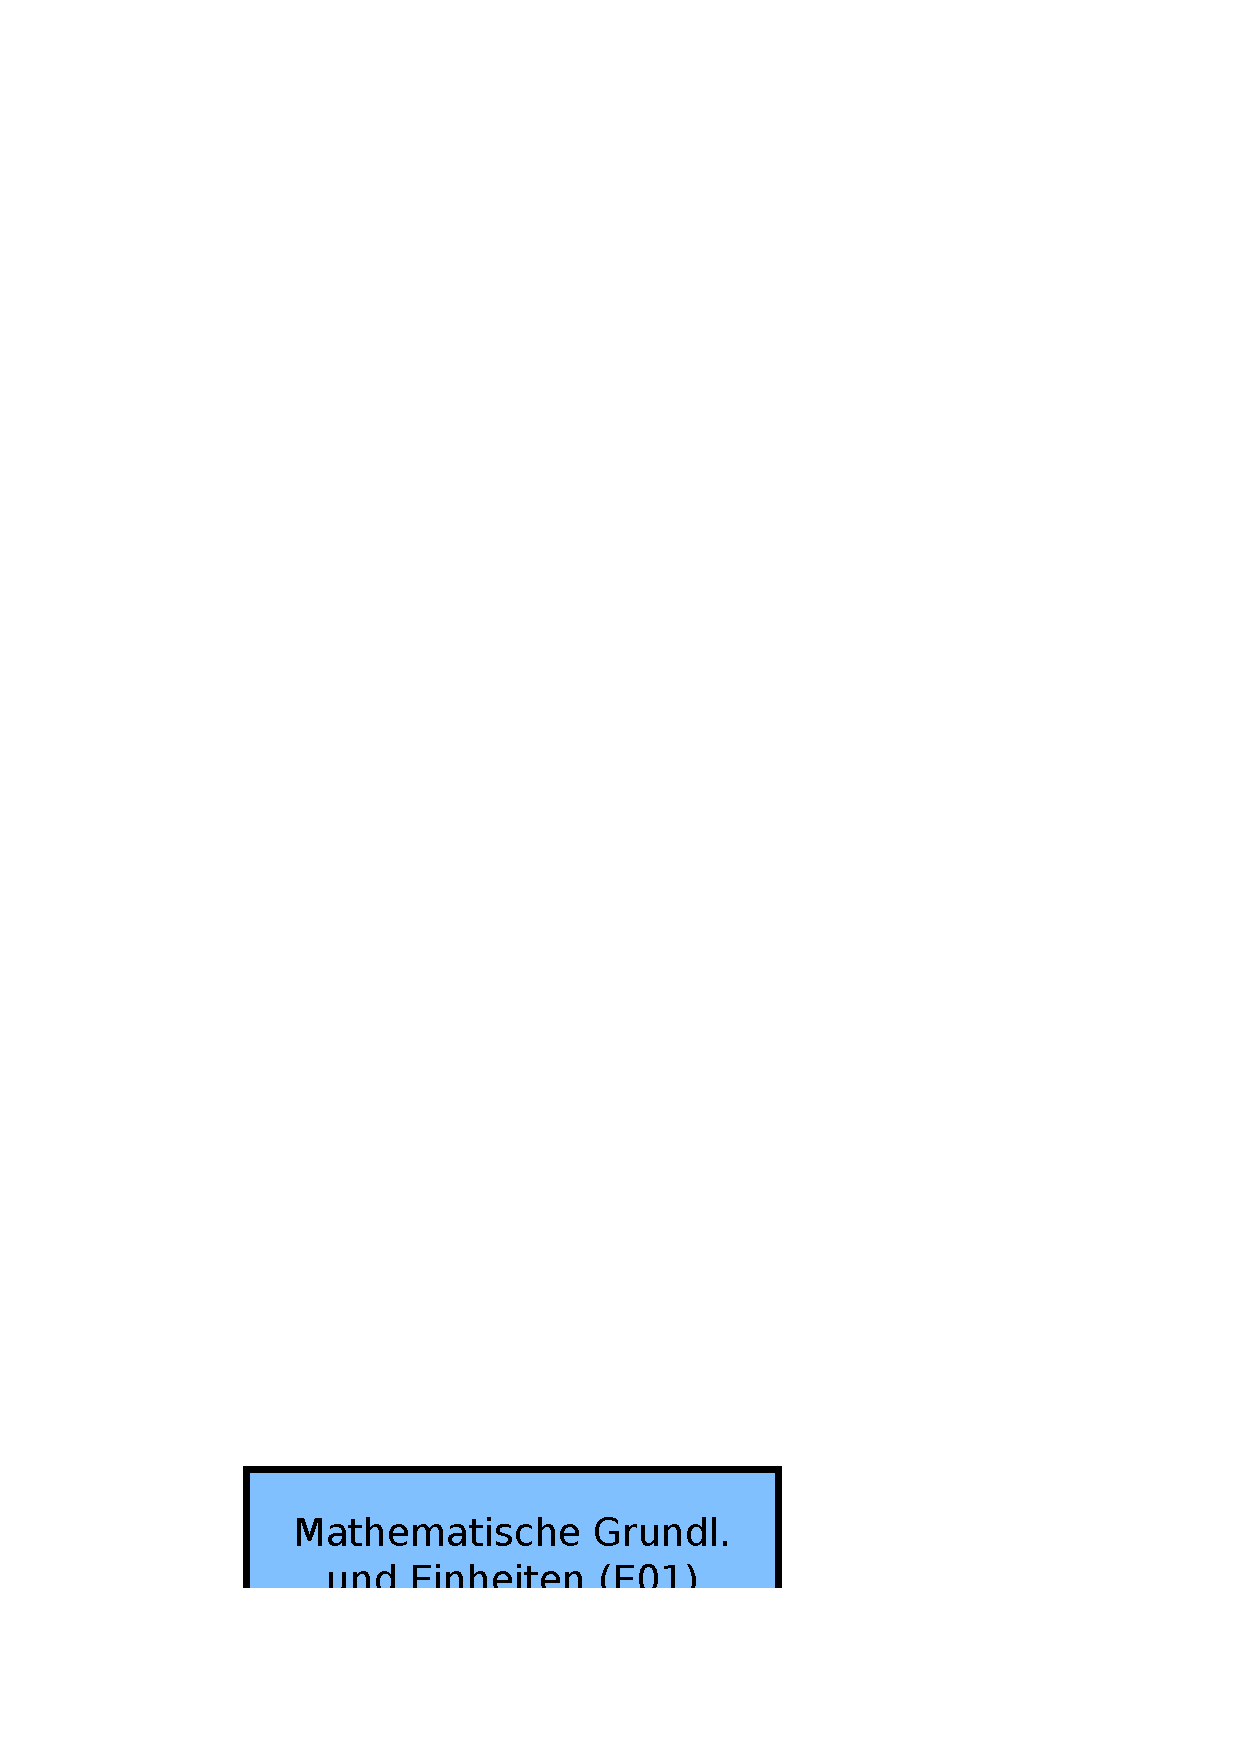
\includegraphics[width=1\textwidth]{o00/Abhaengigkeitsgraph.pdf}

\end{frame}

\begin{frame}
    \frametitle{Curriculum / Lehreinheiten}

    Die genaue \textbf{Aufteilung der Lektionen in 12 bis 13 Lehreinheiten}
    ändert sich immer mal wieder etwas. Der Arbeitsstand kann auf der Website
    zum Kurs \hyperlink{refs}{\cite{curr}} nachgeschlagen werden. \\[2em]

    Dort verlinkt sind zu jeden Thema:

    \begin{itemize}
        \item zusätzliche Anmerkungen\footnote{die noch nicht den Weg in die
              Folien gefunden haben}
        \item entsprechendes Moltrechtkapitel
        \item Foliensatz als PDF
        \item Dateien für Prüfungslerntools mit allen Fragen bis zu dem Stand
        \item kurze Vorbereitungsaufgaben oder Notizen
    \end{itemize}

\end{frame}

\subsubsection{Zeiten}

\begin{frame}
  \frametitle{Kursabend}

  \begin{itemize}
    \item Geöffnet ab ca. 17:45 Uhr
    \item Beginn: 18 Uhr
    \item Zwischendurch eine kurze Pause
    \item Ende der Theorie: 20 Uhr
    \item Danach Amateurfunkabend, manchmal mit Vorträgen und Workshops
  \end{itemize}
\end{frame}

\begin{frame}
  \frametitle{Laufzeit}

  Für Klasse E und Klasse A jeweils 14 Unterrichtseinheiten á 2 Stunden $\Rightarrow$ 28 Stunden\footnote{Plant noch mehr Zeit zum eigenständigen Lernen ein}

  Klasse E vom 18. September bis 18. Dezember

  Klasse A vom 8. Januar bis 16. April
\end{frame}

\subsubsection{Praxis}

\begin{frame}
    \frametitle{Praxis}

    Der Lehrstoff wird manchmal mit einem Praxisthema aus dem Bereich des Afu
    verbunden. Grundsätzlicher Ablauf:

    \begin{itemize}
        \item Betriebstechnik/Vorschriften
        \item Technik Klasse E
        \item Praxis
    \end{itemize}
\end{frame}

\begin{frame}
  \frametitle{Ausflüge für mehr Praxis}

  Wir planen wie im letzten Jahr wieder verschiedene Ausflüge:

  \begin{itemize}
    \item Andere Clubstationen
    \item Sender- und Funktechnikmuseum Königs Wusterhausen
    \item 34. Chaos Communication Congress in Leipzig
    \item CQ TU Contest
    \item Mehrtägige Kursfahrt an einen funktechnisch ruhigen Ort in Brandenburg
    \item EasterHegg 2018 in Würzburg
    \item \ldots
  \end{itemize}
\end{frame}


\subsection{Weitere Quellen}

\subsubsection{Bibliothek}
\begin{frame}
    \frametitle{Weitere Quellen / Bibliothek}

    Neben dem naheliegenden Kauf in einer Buchhandlung, haben viele Bibliotheken
    wie die \emph{UB der TU Berlin} \hyperlink{refs}{\cite{ub}} einiges zum Thema
    Amateurfunk anzubieten.

\end{frame}

\subsubsection{WWW}

\begin{frame}
    \frametitle{Weitere Quellen / WWW}

    \begin{exampleblock}{}
      "`Das Internet ist ein großer Misthaufen, in dem man allerdings auch kleine
      Schätze und Perlen finden kann."' \hyperlink{refs}{\cite{quote}} \\[1em]
      \flushright --Joseph Weizenbaum \\[4em]
    \end{exampleblock}

    \center Wo soll man da nur anfangen?

\end{frame}

\begin{frame}
    \frametitle{WWW}

    Für den Amateurfunkkurs haben wir bereits ein wenig
    Material \hyperlink{refs}{\cite{mat}} zusammengestellt. Für die schnelle
    Suche ist die Wikipedia \hyperlink{refs}{\cite{wp}} ein guter Ausgang. \\[2em]

    Wir haben auch weiterführende freie Inhalte \hyperlink{refs}{\cite{fi}}
    verlinkt. Und ansonsten wie gewohnt die \$SUCHMASCHINE eurer Wahl.

\end{frame}

\subsection{Kosten}

\begin{frame}
  \frametitle{Kosten und Mitgliedschaft}

  Der Kurs an sich ist kostenlos, aber werdet bitte Mitglied im DARC.

  Regulär monatlich 8 EUR.
\end{frame}

\begin{frame}
  \frametitle{Sonstige Kosten}

  \begin{columns}
    \column{.55\textwidth}
    \begin{description}
      \item[Prüfung Klasse E:]80~EUR
      \item[Prüfung Klasse A:]110~EUR
      \item[Rufzeichenzuteilung:]70~EUR
      \item[Frequenznutzung und EMV/U:]ca. 25-30~EUR jährlich (Abrechnung alle 2 bis 4 Jahre)
      \item[Ausflüge:]Diverse Eintritte oder die Kursfahrt (ca. 85 EUR inklusive Mahlzeiten)
      \item[Technik:]Da lässt sich viel ausgeben -- oder selbst bauen
    \end{description}

  \column{.4\textwidth}
    \begin{center}
      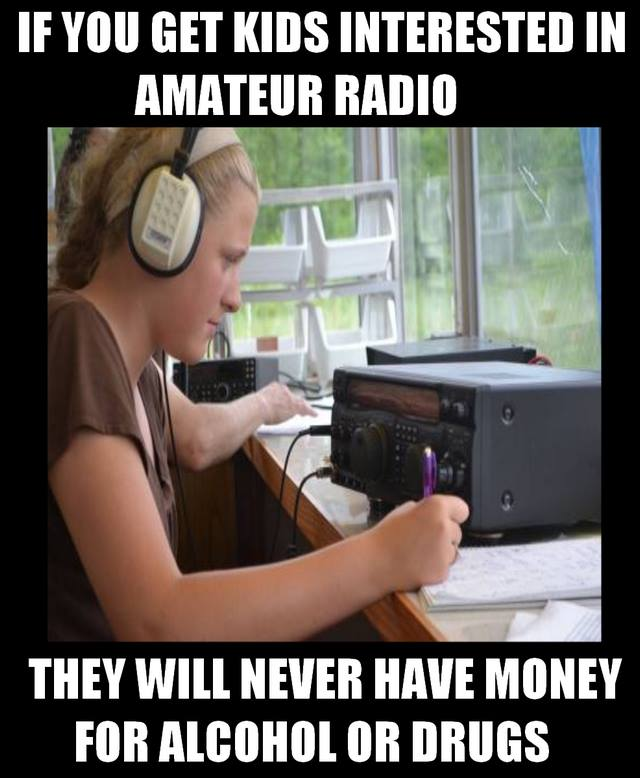
\includegraphics[width=\textwidth]{o00/nomoney.jpg}
    \end{center}
  \end{columns}
\end{frame}

\subsection{Fragen}

\begin{frame}
    \frametitle{Last-but-not-least}

    Disclaimer: Der Kurs findet sich in stetiger Entwicklung.

    \bigskip
    \pause

    Seid ihr bei uns angemeldet? Sonst keine Infos.

    \bigskip
    \pause

    Fragen?

\end{frame}

\renewcommand{\refname}{Referenzen}

\hypertarget{refs}{}
\textcolor{white}{} \\ %\vspace{} geht nicht
\Large Referenzen/Links
\footnotesize

\begin{thebibliography}{}
    \bibitem{meph}  \emph{Originalquelle existiert nicht mehr}
    \bibitem{darc}  DARC Online-Lehrgang Klasse E:
                    \url{http://www.darc.de/referate/ajw/ausbildung/darc-online-lehrgang/technik-klasse-e/}
    \bibitem{dj4uf} Amateurfunklehrgang Betriebstechnik und Vorschriften (E. Moltecht): \\
                    ISBN 978-3-88180-803-3 \\
                    Amateurfunklehrgang Technik Klasse E (E. Moltecht): \\
                    ISBN 978-3-88180-364-9
    \bibitem{curr}  Unterrichtsplan Chaoswelle Kurs: \\
                    \url{https://www.chaoswelle.de/Lehrgang_Berlin_2017/Unterrichtsplan}
    \bibitem{darcv} DARC Verlag:
                    \url{http://darcverlag.de/Amateurfunklehrgang-Technik-fuer-das-Amateurfunkzeugnis-Klasse-E}
    \bibitem{mat}   Material und Dokumente für den Kurs:
                    \url{https://www.dk0tu.de/Kurse/AFu-Lizenz#material}
    \bibitem{afut}  AFUTrainer von DM1OLI:
                    \url{http://www.oliver-saal.de/software/afutrainer/}
    \bibitem{afutest}  AFu-Test von DD6EE:
                    \url{https://afutest.ewers.net}
    \bibitem{afup}  Prüfungen zum Amateurfunkzeugnis vom Ortsverband A36:
                    \url{http://www.afup.a36.de/pruefungen/pruefungen.html}
    \bibitem{ub}    Universitätsbibliothek der TU Berlin:
                    \url{http://www.ub.tu-berlin.de}
    \bibitem{quote} Joseph Weizenbaum, aus Wikiquote:
                    \url{http://de.wikiquote.org/wiki/Joseph_Weizenbaum}
    \bibitem{wp}    Wikipedia - Die freie Enzyklopädie:
                    \url{http://www.wikipedia.org/}
    \bibitem{fi}    Freie Inhalte (DK0TU):
                    \url{https://www.dk0tu.de/Projekte/Freie_Inhalte/}
\end{thebibliography} 

% Hier könnte noch eine Kontaktfolie stehen

\end{document}

